\documentclass[a4paper,11pt,parskip,abstract=on,thesis,DIV=9]{scrreprt}
% \documentclass[a4paper,11pt,abstract=on]{report}
\usepackage[T1]{fontenc}
\usepackage[utf8]{inputenc}
\usepackage{lmodern}
\usepackage{mathptmx}
\usepackage[page]{appendix}
\usepackage{listings}
\usepackage{color}
\usepackage{pdfpages}
\usepackage{lipsum}
\usepackage{float}
\usepackage{textcomp}
\usepackage[english]{babel}
\usepackage{csquotes}
\usepackage{caption}
\usepackage[style=apa,citestyle=apa,backend=biber,hyperref=true,apabackref=true]{biblatex}
\usepackage{hyperref}
\usepackage{doi}

\DeclareLanguageMapping{english}{english-apa}

\addbibresource{final_report/bibliography.bib}
\setkomafont{disposition}{\normalfont\bfseries}

\definecolor{mygreen}{rgb}{0,0.6,0}
\definecolor{mygray}{rgb}{0.5,0.5,0.5}
\definecolor{mymauve}{rgb}{0.58,0,0.82}

\lstset{frame=tb,
  aboveskip=3mm,
  belowskip=3mm,
  backgroundcolor=\color{white},   % choose the background color; you must add \usepackage{color} or \usepackage{xcolor}; should come as last argument
  basicstyle={\small\ttfamily},    % the size of the fonts that are used for the code
  breakatwhitespace=true,          % sets if automatic breaks should only happen at whitespace
  breaklines=true,                 % sets automatic line breaking
  captionpos=b,                    % sets the caption-position to bottom
  commentstyle=\color{mygreen},    % comment style
  columns=flexible,
  frame=single,	                   % adds a frame around the code
  keepspaces=true,                 % keeps spaces in text, useful for keeping indentation of code (possibly needs columns=flexible)
  keywordstyle=\color{blue},       % keyword style
  language=Python,                 % the language of the code
  numbers=left,                    % where to put the line-numbers; possible values are (none, left, right)
  numberstyle=\tiny\color{mygray}, % the style that is used for the line-numbers
  rulecolor=\color{black},         % if not set, the frame-color may be changed on line-breaks within not-black text (e.g. comments (green here))
  showspaces=false,                % show spaces everywhere adding particular underscores; it overrides 'showstringspaces'
  showstringspaces=false,          % underline spaces within strings only
  showtabs=false,                  % show tabs within strings adding particular underscores
  stepnumber=1,                    % the step between two line-numbers. If it's 1, each line will be numbered
  stringstyle=\color{mymauve},     % string literal style
  tabsize=2,	                     % sets default tabsize to 2 spaces
}

\renewcommand{\lstlistingname}{Code}

\subject{Computer Science Final Year}
\title{Evaluation of a Haskell Web Framework}
\author{Junaid Ali Rasheed}


\begin{document}
\pagenumbering{roman}


\maketitle

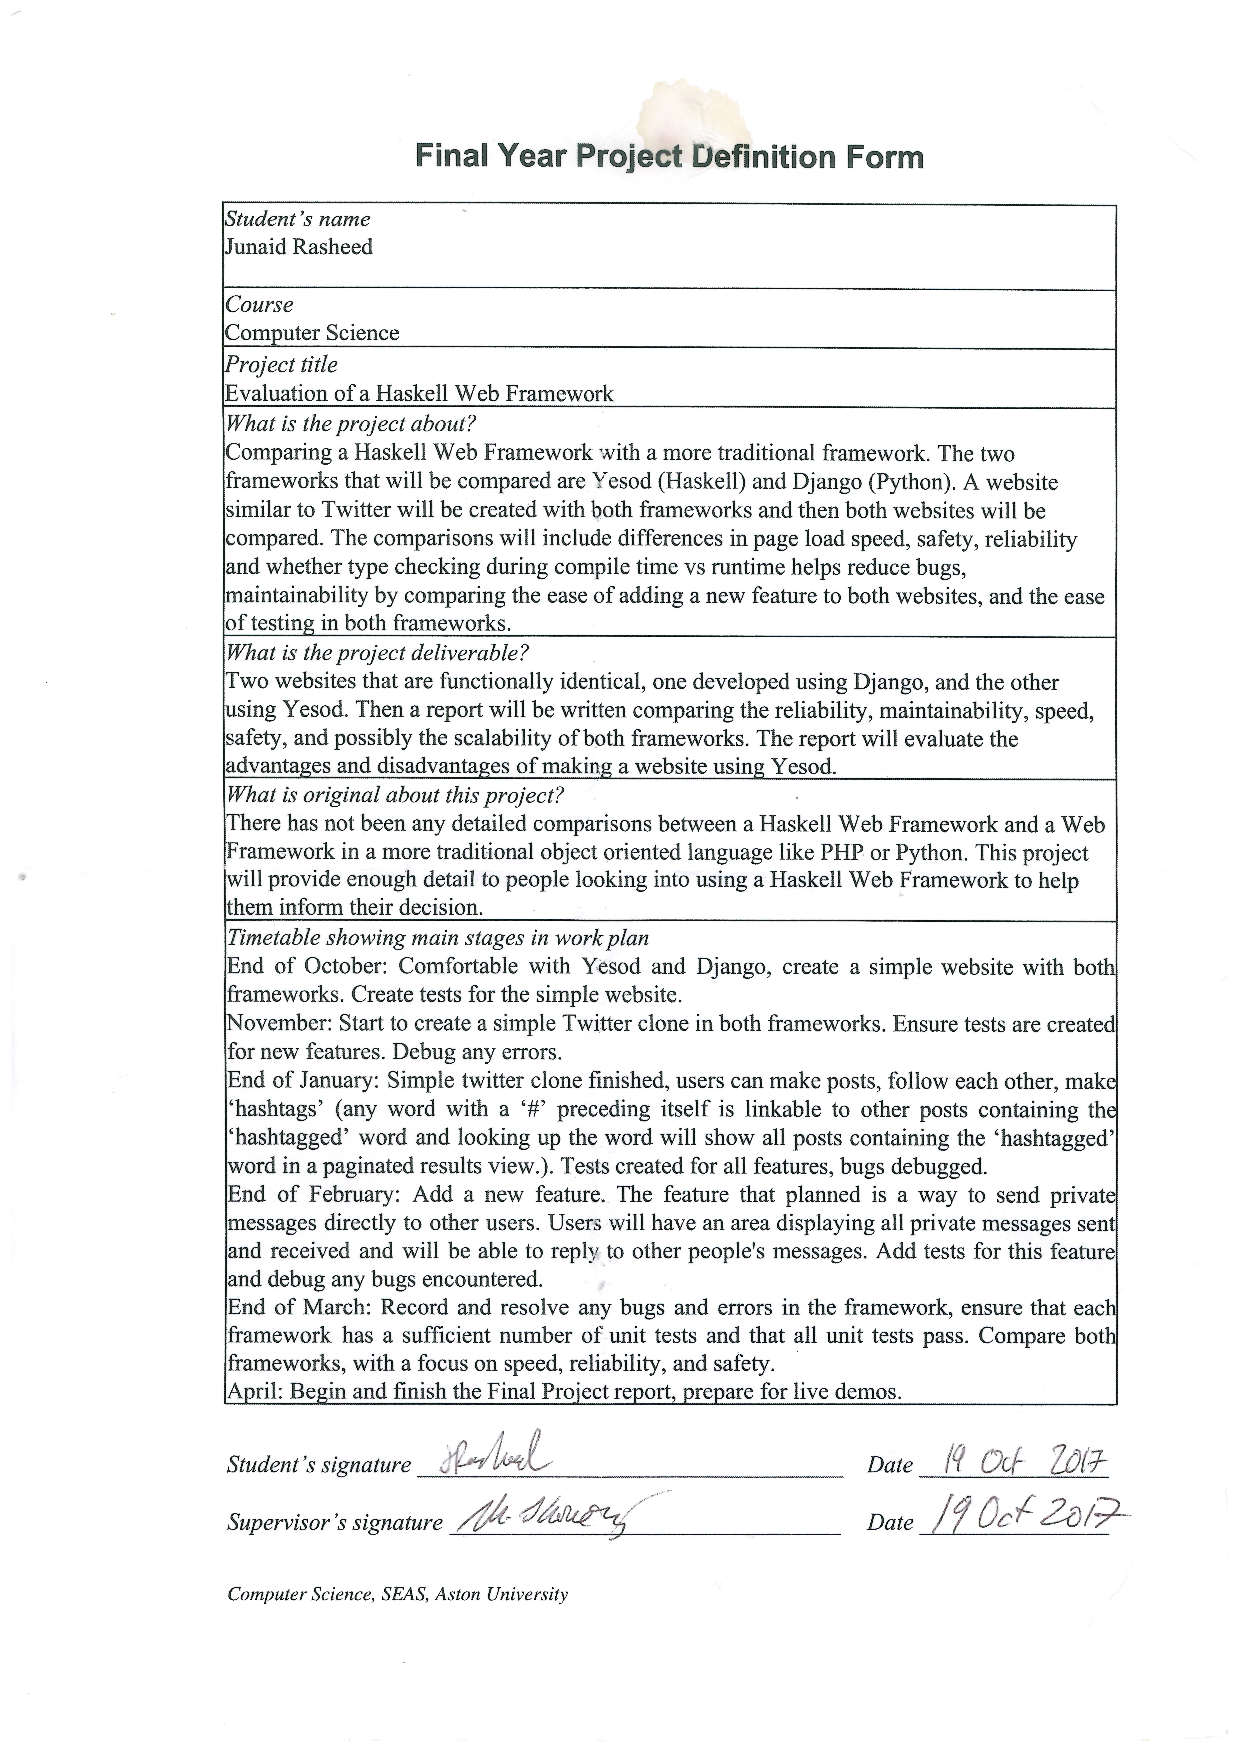
\includepdf[pages=-]{pdf_documents/Final_Year_Project_Definition_Form_Signed.pdf}

\tableofcontents
\listoffigures

\begin{abstract}
\lipsum[1-3]
\end{abstract}

\pagenumbering{arabic}

\chapter{Introduction}

In this report, we will compare two web frameworks, one written in Haskell and another, more
popular framework, written in a typical object oriented language. To perform the evaluation,
a functionally identical website was created in both frameworks.

One issue that individuals face when looking into Haskell Web frameworks is the lack of
detailed comparisons between these frameworks and more traditional frameworks that these
individuals likely have experience in. This report will provide an in-depth look at the
advantages and disadvantages of choosing to use a Haskell Web Framework, and will help
these individuals come to an informed decision on whether or not a Haskell Web Framework is
best for them.

\section{The Chosen Frameworks}

Yesod is a fully featured and modular web framework written in Haskell. Yesod claims to use
features of the Haskell language to provide a fast, modular, and type safe web framework. By
choosing Yesod as the web framework for the Haskell language, we will be able to determine
whether or not Haskell's type safety, referential transparency, and lazy compiling is an advantage
or a disadvantage for web developers.

\begin{quote}
Yesod attempts to ease the web development process by playing to the strengths of the Haskell 
programming language. Haskell’s strong compile-time guarantees of correctness not only encompass 
types; referential transparency ensures that we don’t have any unintended side effects. Pattern 
matching on algebraic data types can help guarantee we’ve accounted for every possible case. 
By building upon Haskell, entire classes of bugs disappear. \parencite[Introduction]{yesodBook}
\end{quote}

Django is a Python Web Framework. Django, like Yesod, is a ``batteries included'' web framework,
``instead of having to open up the language to insert your own power (batteries), you just have
to flick the switch and Django does the rest.'' \parencite{djangoBookReasons}. I chose Django
for a number of reasons

\begin{itemize}
  \item ``Batteries included'', like Yesod
  \item Modular, like Yesod
  \item Python is now more common than PHP, second only to Node.js \parencite{djangoBookReasons}
\end{itemize}

The Django and Yesod web frameworks have a similar set of features. This ensured that we could
make a functionally identical site in both of these frameworks with a similar 
amount of effort. This enables us to make a fair comparison between Django and Yesod, enabling
us to come to a conclusion on whether a Haskell web framework may be a good choice for a 
developer rather than a more tradition web framework.

\section{The Report}

The rest of this report will discuss any pieces of work similar to this project, the process of
writing the code for both frameworks, including any preparation that had to be done, and a detailed
evaluation of the websites that were produced. The evaluation will compare page load speeds,
the reliability and maintainability of the websites, the ease of writing new code, the ease of
debugging issues, the features including in each framework's test suite, and whether the static typing
and type safety of the Haskell language help or hinder the process of developing a website.
\chapter{Background}
\label{chap:Background}

In this chapter, we will discuss previous work and research pertaining
to Haskell web frameworks and any real-world sites built using a Haskell
web framework.

\section{Similar Previous Work}

Looking through scientific journals, online articles, and blog posts,
you can find many individuals documenting their experiences and performing
reviews of Haskell Web Frameworks. For example, in the IEEE Internet Computing
journal, \citeauthor{snapFramework} have written an article giving an overview
of Snap. According to the article, snap is a simple web framework written
in Haskell where programming is done at a similar level of abstraction
to Java servlets. The article instructs the reader on how to install Snap, 
walks the reader through some sample code, and shows a quick comparison
between Snap and other major web frameworks. The comparison is a benchmark
of each framework, recording the amount of time it takes for each framework
to respond to a request. The benchmark results can be seen in Figure 
~\ref{fig:snapBenchmark}. \parencite{snapFramework}

\begin{figure}[H]
    \centering
    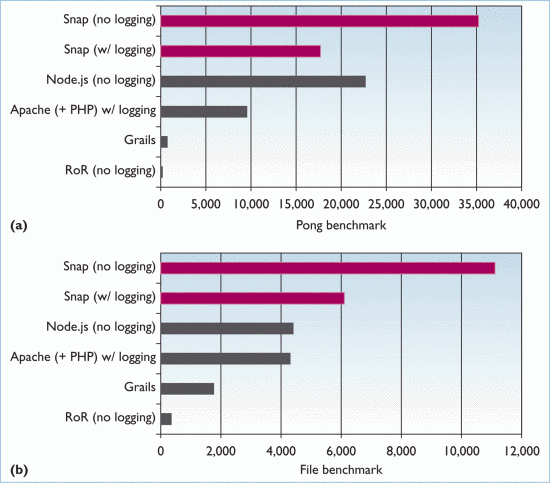
\includegraphics[width=0.7\textwidth]{final_report/pics/snapBenchmark.png}
    \caption{Snap and other frameworks, values are in requests per second \\ \textcopyright{} \citeyear{snapFramework} IEEE}
    \label{fig:snapBenchmark}
\end{figure}

Figure ~\ref{fig:snapBenchmark} shows the results of two benchmarks, one where a server
responded to a request by sending the string "pong", and another that records how fast
a server can send a 49 kilobyte image. As you can see in the
graph, for the file benchmark, the Snap framework was faster than all other frameworks.
Snap was only beaten by Node.js in the Pong benchmark when logging was turned on.
Turning logging off dramatically increased the performance of Snap, resulting in
Snap being 55\% faster than Node.js in the Pong benchmark. \parencite{snapFramework}

So, from the research done by \citeauthor{snapFramework}, we can see that Haskell
web frameworks can be significantly faster than more traditional web frameworks.
This is because Haskell uses the Glasgow Haskell Compiler (GHC). GHC compiles
Haskell programs into native machine code, ensuring high performance, especially
for concurrent programs such as web servers. Because of this, any Haskell web framework
that uses GHC, including Yesod, will serve requests faster than most traditional
web frameworks. \parencite{ghcSite}

\citeauthor{haskellWebComparison} published a blog post on his website with the
title \citetitle{haskellWebComparison}. In the post, \citeauthor{haskellWebComparison}
provides a quick comparison between some popular Haskell Web Frameworks, including
Yesod and Snap. The comparisons include the installation process of each framework,
the way they handle routing -- i.e. pointing a URL to a piece of code that will 
produce a response, and the quality of documentation for each framework. \parencite{haskellWebComparison}

At the end of his comparison, \citeauthor{haskellWebComparison} found that Yesod
was the best framework for his use case. One of the reasons for his choice was
because of the great documentation available for Yesod. The creator of Yesod
has written a book, \citetitle{haskellBook}, that is very comprehensive. The book
is available for free on the Yesod website. The amount of detail contained in this
book is also one of the reasons the Yesod web framework was chosen for this
project. \parencite{haskellWebComparison,yesodBook}

In \citetitle{beginnerYesod}, \citeauthor{beginnerYesod} discusses his experiences
in using Yesod as a beginner to the Haskell programming language. He mentions
the depth and thoroughness of the Yesod book when learning Yesod. However, when
making an actual website, he came across difficulties when trying to implement
features that required the use of functions not in the book. The author had
to check the documentation of the functions on Hackage, a Haskell package archive.
On Hackage, most functions contain a type signature and normally a one line
description. The author mentions how the type signatures would probably be
enough for experienced Haskell developers to work out how to use a function
but, as a beginner, founding out how a function works using types was much more
difficult. Because of this, the author had to spend a lot of time fixing type
errors. \parencite{beginnerYesod}

When first starting the project, I personally experienced the same issues described
in \citeauthor{beginnerYesod}'s blog post. I was not very good at reading the type
signatures available on Hackage, resulting in spending a lot of time fixing
unmatched type errors when trying to use functions not documented in the book.
However, as I became more experienced in Yesod and Haskell, these problems
became more and more rare as my understanding of Haskell type signatures increased.

\section{Real World Haskell Sites}

Some readers will be concerned about whether or not a Haskell web framework like
Yesod is ready for production websites. This is a valid concern considering the
relatively small amount of Haskell programmers when compared to mainstream 
programming languages. Readers will be pleased to know, however, that there
are some high traffic sites that are built using the Yesod web framework.

Freckle, previously known as Front Row Education, is an education
platform that provides a service to almost 10 million students \parencite{frontrowName}. 
In 2015, Freckle migrated their site to the Yesod web framework and have been 
using it ever since. \citeauthor{frontrow}, the CTO of Freckle, wrote an article
on his experience of using Yesod for a high traffic website. \parencite{frontrow}

In his article, \citeauthor{frontrow} states that the reason they chose a Haskell
Web Framework was because of the low resource usage and the ability to make
quick iterations that the Haskell language gives you. The article also discusses
how static typing saves time when writing unit tests. The developers at Freckle
did not have to deal with checking for null exceptions, mismatched types, and
other common bugs that are annoying to deal with. Spending less time dealing with
dynamic typing gives developers more time in implementing their features. The
modularity of Yesod also allows Freckle to reuse complex code, reducing potential
mistakes by developers, reducing the amount of code that needs to be written,
and allowing code to be updated quickly without the need to repeat changes. All
of these advantages allow developers to be more efficient and write fewer bugs. \parencite{frontrow}

However, there are some issues that the Freckle team came across during their migration.
Haskell builds are normally quite slow, as all external libraries used have to be
compiled during the build process. \citeauthor{frontrow} mentions that builds took
5-10 minutes on their most powerful machines. The author does mention that the team
could improve their build process by, for example, caching built files. The testing
suite caused problems for the team because when a test fails, they could not determine
which condition caused the failure when a test block has multiple conditions. The issue,
however, was reported to developers behind the testing library and the current
version of the testing suite does not have the issue mentioned in the article. The
lack of documentation for some functions also caused some frustration to the development
team, especially for the more junior developers who could not rely on type signatures. \parencite{frontrow}

When Freckle switched their main API to Yesod, their CPU usage rose to 95\%. This issue
did not occur during testing and profiling, in fact, the Freckle team were the first to
experience this particular issue. This is one issue when using a relatively niche language
like Haskell, you have to be comfortable with the idea that you may be the first person
to experience a particular issue. With other popular frameworks like Django, any issue
you discover has most likely been found and fixed by other members of the community.

Despite these issues, Freckle decided to stick with Yesod due to the advantages of the
Haskell compiler and the fact that the issues they experienced with regards to documentation
and build time are improving. And although the community is small, you can almost
always find help by asking on the StackOverflow or Google Groups pages or by visiting
the \#haskell-beginners IRC channel, an online chat room where developers new to Haskell
can quickly and easily get help from some more experienced developers.

%\chapter{Preparation}
\label{chap:Preparation}

In this chapter, we will discuss the work that needed to be done before work could
be started on developing websites in Yesod and Django.

\section{Planning the Website}

Before any work was done, a plan was created that indicated the features the
website should contain to ensure that the each framework is tested and
evaluated fairly. The website to be created was a twitter
clone with the following features: a home page, authentication, a profile page,
ability to post a message, ability to post `tagged' messages (any words with
a preceding `\#' becomes link that leads to a search page),
ability to search for messages and users, and an ability to follow other users.
All features implemented would also have unit tests implemented using the
testing tools available in each framework. After each site is feature complete,
a new feature, the ability to message other users, should be implemented.

Implementing these features allows us to test page load speed by navigating
to certain web pages. We can evaluate how the static type checking and type safety features of 
Haskell affects reliability when compared to dynamic type checking in Python. Testing
all of our implemented features allows us to fairly evaluate the
test suites included with each framework. Implementing a new feature once each
site is feature complete will also allow us to test the maintainability of
each framework.

By planning the website before any work was done, there was a clear vision of
what the website should look like. This allowed development to focus on implementing
the specified features rather than trying to design new features while developing
at the same time, ensuring that functionally identical websites are created in both
frameworks that can be fairly compared and evaluated.

\section{Learning the Frameworks}

Even after the planning was completed for both sites, before any development could
be done, the basics of each framework must be learned. This ensures that code
produced follows the latest standards of each framework, the built-in features
of each framework that may help with development are understood and used appropriately,
and code produced is of a high standard, maintainable, and readable.

\subsection{Learning Django}

Because of previous experience with Python and other object oriented web frameworks, 
Django was learned quickly by going through the official Django tutorials and 
documentation.

The Django tutorials themselves were straight forward for someone who has 
experience in Python and other web frameworks. The tutorials walk you through
installing Django and creating your own app. In Django, an app resides in a project
and is a web application that performs some function. An example of an app could be
a web blogging system. A Django project is a collection of apps and configuration
settings for a particular website. After completing the Django tutorials, work
on the planned website was begun. \parencite{djangoIntroDocs}

\subsection{Learning Yesod}

Coming from an object oriented background, it was not trivial to start using
a functional programming language like Haskell. Before development with the
Yesod framework could be started, the Haskell language had to be learned to
an adequate level.

To help with learning Haskell, the book \citetitle{haskellBook} \parencite{haskellBook}
was used. This book walks the reader through learning the Haskell language beginning
with the fundamentals. Reading through several chapters of the book gives
the reader a basic understanding of programming with Haskell, allowing the reader
start learning Yesod itself, referring to the book to understand more
advanced concepts as you come across them.

To learn Yesod, the book \citetitle{yesodBook} \parencite{yesodBook}, 
written by the person who wrote Yesod, was used. The book goes through all of the
features of the Yesod framework in an easy to understand manner. After
reading the book, development on the planned website using the Yesod
framework was started.

\section{The Evaluation}

Once the website was feature complete on both frameworks, a series of experiments
were ran to compare the features that we planned to test during the planning phase.
The raw data of these experiments can be found in the appendix and an evaluation
of these results are discussed in the next chapter.

%\include{final_report/4_delivarable}
%\chapter{Evaluation}
\label{chap:Evaluation}
%\chapter{Conclusion}

In this report, we have discussed how we evaluated a
Haskell web framework. We compared two frameworks,
a Haskell framework called Yesod, and a Python
framework called Django. We gave a high-level explanation
of how the two frameworks worked. We explained the preparation
needed before development could be started in both frameworks.

Once the websites were complete, we performed tests to compare
each framework. These tests were used to: evaluate the performance
of each framework, compare how the language features
of each framework help or hinder web development, and test
the resource efficiency of each framework. After performing
these tests and discussing the results, we wrote a section
that discussed who we would recommend the Yesod framework
to. Overall, Yesod is a production ready framework that is
ready to be used (and has been used), in the real world.

Personally, this project has greatly improved my own academic and
development skills. I gained a lot of knowledge of the Haskell
programming language by getting some hands on experience with
Yesod, a framework that uses a lot of advanced features of Haskell.
By writing this report, my academic
research and writing skills have greatly improved, as I had to
perform a lot of research on existing scientific journals about
Haskell web frameworks.
I have also made some contributions to open source Haskell projects, and
have become more interested in the academic side of Computer
Science.


\printbibliography[heading=bibintoc,title={References}]

\begin{refsection}
\nocite{*}
\printbibliography[heading=bibintoc,title={Bibliography}]  
\end{refsection}

\begin{appendices}

\chapter{Project Diary}
\section{Meeting 1 - 3rd October 2017}

\subsection{Meeting Notes:}

\subsubsection{Books}

Real World Haskell\\
Haskell from first principles (haskellbook.com)\\
Web application development with Haskell and Yesod (out of date)

\subsubsection{Frameworks / Tools}

Haskell Servant package\\
Snap is alternative to Yesod\\
ghcjs haskell to js\\
haskell stack tool\\
hackage is like npm. Stack can use hackage.\\
Stackage is like stack on top of hackage\\
Use the latest LTS version of haskell from stackage\\
Atom could be useful with their plugins, compare with plugins available for code\\
ghc-mod available for haskell in atom, helpful when developing\\
ide-haskell, linter\\
There is a Haskell plugin for intellij which may work. Good because I would be familiar with the IDE.

\subsubsection{Comparing the two frameworks}

\begin{itemize}
  \item Maintainability
  \begin{itemize}
    \item Make a change to both
  \end{itemize}
  \item Performance
  \item Scalability - could use tools, hard to do on your own
  \item People say Haskell is easier to write code with, less time debugging, once learnt
  \begin{itemize}
    \item We could test this. How much the type checking helps. The different tools available
    \item Can't use line by line debugging
  \end{itemize}
\end{itemize}

\subsubsection{Plan for next meeting}

Do as much as possible for now\\
Come up with rough project definition form\\
Go through some haskell tutorials, haskellbook.com is recommended

\section{Meeting 2 - 12th October 2017}

\subsection{Meeting Notes:}

Look into getting GHC mod compile on save\\
Get the project proposal doc ready for next week\\
Learn Django and get it installed on the laptop\\
Make a basic page in Django and Haskell

\section{Meeting 3 - 19th October 2017}

\subsection{Meeting Notes:}

Carry on with the Haskell Programming from First principles book\\
Have some planning for the twitter clone ready

\section{Meeting 4 - 24th October 2017}

\subsection{Meeting Notes:}

Set up a basic homepage in Yesod and Django. Do this over the weekend.\\
Have a play around with the yesod site that’s provided to see what you can focus on.\\
Carry on with the book\\
Setup Docker/Vagrant if you have time at the end, for instructions on setting up the repo\\
Topics important for yesod
\begin{itemize}
  \item Quasi quotes, provided by yesod
  \item Yesod Typeclass could be useful to know
\end{itemize}

\section{Meeting 5 - 10th November 2017}

\subsection{Meeting Notes:}

I’ve created the homepages in both yesod and django. I’ve used tests in django to test a basic app not related to the project

Next week, I want to ensure both home pages are the same and to create tests in both frameworks. I want to progress more through the yesod and haskell book.
Create User models in both yesod and django and create tests for them.

\section{Meeting 6 - 16th November 2017}

\subsection{Meeting Notes:}

I’ve created the homepages in yesod and django and ensured that they both have the same content and styling.

For django, I have added the functionality to allow users to create accounts and log in. I have added unit tests for this and they all pass.

For yesod, I have added the latest version of jquery and bootstrap to the project. I have tried to complete the user account functionality but I am blocked. I am trying to import yesod-auth-hashdb but cannot figure out how to do it. There is some documentation showing how to edit the cabal file but this is overwritten during the build, I believe the data comes from package.yml. Editing package.yml causes strange errors when I try to build the project but I don’t think I am doing it in the correct manner. Need to figure out how to edit the package.yml, edits would result in errors on my computer.

For next week, I want to fix the weird error and get some tests up.

Things to try to resolve the error, try to reproduce it on normal ubuntu. If you can’t resolve it, report it to yesod.

\section{Meeting 7 - 23rd November 2017}

\subsection{Meeting Notes:}

I’ve resolved the random error we had last week.\\
I’ve imported hashdb and have added functionality for users to create accounts and login on the yesod site.\\
Yesod forms rely on bootstrap 3, so downgraded from bootstrap 4 (beta) to 3.

For next time...\\
I want to figure out how to concatenate a Text data variable in Yesod. Have to figure out how to deal with overloaded strings?\\
Finish the user authentication functionality. Show appropriate messages and add extra validation to the yesod form (unique user and email, min and max length of fields).\\
Create tests for the user authentication functionality.\\
Change the forms on Django to use their form model rather than a HTML form. This will let me compare the pros and cons of Django’s and Yesod’s forms.\\
If there is time, add functionality to allow users to post messages. These messages should be saved in the database so that the user can see all the messages they’ve posted when they log in.

The user post message page should use ajax so when they post a message, the part of the div will just reload rather than the whole page.

\section{Meeting 8 - 14th December 2017}

\subsection{Meeting Notes:}
On the yesod site:\\
Have some tests working\\
Users can post messages, be signed up, see other users messages\\
Have some tests working, this is WIP

For next time…\\
Get Django messages working\\
Try to get ajax working on both sites, see https://www.yesodweb.com/blog/2013/02/ajax-with-scaffold

Interim report plan
\begin{itemize}
  \item Intro
  \item Explain the choices of yesod and django
  \item Do some initial comparisons of the site
  \item My experiences with developing on both sites, what I found easy and hard on the different frameworks.
  \item Advantages and disadvantages of both frameworks.
\end{itemize}

\section{Meeting 9 - 1st February 2018}

\subsection{Meeting Notes:}
Worked mainly on the Django site. I have the messages working and have began comparing features between two sites such as
\begin{itemize}
  \item The implementation of Handlers/Routes
  \item The way you can pass variables to templates
  \item How Haskell's 'maybe' reduces the number of errors you need to catch
  \item the ways you can implement AJAX in both frameworks
\end{itemize}

In the near future, refactor the messages implementation to use AJAX for retrieval of messages and creating new messages. This refactoring will help compare the ease of modifiability of both of these frameworks.\\
Whenever you come across a difficult error, try to compare the process of debugging in both frameworks.\\
Remember to focus on using different parts of the framework than just implementing new features on the site.\\
Try to resolve the textarea problem. If you can't send a screenshot of the error.\\

\section{Meeting 10 - 15th February 2018}

\subsection{Meeting Notes:}
Created AJAX functionality for getting messages

Resolved issue with using single template for profile by declaring the form stuff even if isCurrentUse is false, this is fine

\subsubsection{What needs to be done}

Add more tests this weekend for both frameworks. Does Haskell's type checking mean we need fewer tests compared to Python?

\subsubsection{What to look at for evaluation}

Evaluate:
\begin{itemize}
	\item{The ease of writing tests}
	\item{In python, you need lots of testing because there's no static type checking}
	\begin{itemize}
    	\item{Does this mean you need less tests in Haskell}
    	\item{Does this mean tests are easier to write in Haskell, or in Python because tests are more important in Python so they'd be easier to use}
	\end{itemize}
	\item{What types of tests are important in the haskell world}
	\item{Some tests are unneeded for Haskell}
	\item{Is it cheaper to build a bullet proof app in Haskell or Python, maintainability? etc}
\end{itemize}

Amount of users in Django makes it easier to find problems that others have experineced

Amount of users in Django means more tools for Django but this is improving on the Haskell on the side

The Yesod book written by the creator of Yesod is pretty good

Some of the problems written by people using Yesod are more detailed, users are probably more experienced in the programming world? more academic?

Evaluate the ease of adding a new feature after the site is complete

Evaluate how quick it is to debug something

Built in compiler and type checking in Haskell is very useful when debugging

Evaluate page load speeds, is Python slower because it runs the interpreter every time?

Scalability if you can

Some quantitative data?

Explain to the reader why some things make a big difference
\begin{itemize}
    \item{How long it takes to get a reliable application}
    \begin{itemize}
        \item{Length of tests? Number of tests? Instances where types catch important errors? These are very useful}
        \item{Times where the type checking or other similar features got in your way?}
        \begin{itemize}
            \item{E.g. profile page was easier to code in Python, this was because of Haskell checking the scoping}
		\end{itemize}
	\end{itemize}
\end{itemize}
\section{Meeting 11 - 22nd March 2018}

\subsection{Meeting Notes:}
Implemented type safety for some URLs

\begin{itemize}
  \item{How much does it help with testing / debugging?}
  \item{Does this reduce the amount of code you need (to check parameter types, etc.)}
\end{itemize}

Joins cannot be done with Yesod Persistent (alternative pseudo SQL available) but restructuring
logic may be more efficient than joins.

\subsubsection{Plan for the holidays and beyond}
\begin{itemize}
  \item{Finish the functionality of both websites by the end of week 2 of the holidays}
  \item{Produce a report by the end of week 3 of the holidays}
  \item{Get feedback and produce another version of the report the first week back from the holidays}
  \item{Get more feedback and produce a final version of the report the second week after the holidays}
\end{itemize}

\section{Meeting 12 - 19th April 2018}

\subsection{Meeting Notes:}
Report draft, hand in by this weekend.

Book in a meeting on Tuesday to discuss the report.

Simulate mistakes and see how the Haskell compilers help

Argue against how the compiler may make you write unnecessary code

\begin{itemize}
  \item{Haskell version, I couldn't do something like if not null, ignore the block}
  \item{You can try to use an undefined and force an exception}
  \item{You can do something like ``Error - (loc) shouldn't happen''}
\end{itemize}

Type safety saved a lot of time with checking variable types

But people like python because of the lack of type checking

It may be faster to ignore types when developing but it could cause problems later on

Think about separating language and framework

For this report, it's more useful to focus on the framework, but think about anything to do with the language

For example, static type checking is to do with Haskell rather than Yesod

In the yesod-test package, you can use HTML selectors. That makes testing static content easy.

Django, you can test HTML page but selectors are not implemented. (If html page contains this string).

If you have time after getting the report done...

Load testing, deploy both apps to the same environment. Is there a tool for it. Send 
multiple queries from multiple machines, time responses.

If no tool, you can try requests from just your own machine.
If you can't get it on Heroku, set up a VM.

Test the ease of deployments for both frameworks. Test the actual production mode, not dev mode.

\section{Meeting 13 - 24th April 2018}

\subsection{Meeting Notes:}
Entity relation diagram.

Redo tests on EC2 instances.

For research reports
\begin{itemize}
  \item State objective, hypothesis, search question.
  \item Methodology, development (testing, iterative development, conntinous integration)
  \item Mention websites as explicit deliverables that support the comparison.
  \item Comparison methodology, what do frameworks give you to support TDD.
  \item Evaluation methodology, deploy, page load speeds, load speeds, documentation.
\end{itemize}

Background chapter, expand on Yesod and Django components. 
Some diagrams would be nice.


\section{Meeting 14 - 26th April 2018}

\subsection{Meeting Notes:}


For the networking test where you mention that Django uses more data,
use the network tab on the browser to confirm this. If you load
the site in Yesod, the data loaded is lower and then it's compressed.

Fix lstlisting, set language before code blocks.

When Yesod throws errors, say runtime error, with a compiler message.

texcel, you can use macros. Could make font for code smaller.
Reformat the code blocks to be easier to read.
Any case against the types. Early profile page was one request/view. This meant that
there was some extra Haskell code that had to be written.

Last section, fix typo `Yesod being less resource intensive than Yesod.', wrong
your.

Small section that talks about how you made a functional, actually usable,
site. Site is realistic, which gives us a useful way to evaluate the frameworks.
This could be before the testing method.

Amazon monitoring is only available in five minute intervals (free usage limit).

A refactor at the end would have been useful to evaluate at the end. Does
the more rigid structure of the Haskell program help with refactoring?
Haskell compiler would guide you on what needs to be changed after a
small change.

Conclusion
Summarise the entire report, half a page, a side.

Get rid of some of the more uninteresting website images.

A useful diagram would explain the architecture of each framework.

\section{Project Definition Form}

\subsection{14th October 2017}

First draught written up and sent to tutor via email for feedback

\subsection{15th October 2017}

Tutor feedback implemented

\subsection{19th October 2017}

Tutor and I signed form. Form is submitted electronically via Turnitin

\section{Interim Report}

\subsection{18th January 2018}
Interim report started and then finished

\subsection{19th January 2018}
Sent Ethics form to tutor

Proof-read and submitted the interim report

\section{Software Development}

This section records the development lifecycle of the Django and Yesod sites. More detailed commit messages
can be found by running a \textit{git log} on the git repo for both sites.

\subsection{Yesod Site}

\subsubsection{1st November 2017}
Created a basic homepage and a vagrantfile.

\subsubsection{23rd November 2017}
Implemented Login and Signup functionality

\subsubsection{11th December 2017}
Created a profile page

\subsubsection{14th December 2017}
Implemented message creation functionality and added some tests

\subsubsection{15th February 2018}
Modified profile page to retrieve messages using AJAX

\subsubsection{19th March 2018}
Implemented functionality to show other registered users on the profile page

\subsubsection{20th March 2018}
Basic functionality to follow users implemented

\subsubsection{21st March 2018}
Refactor profle page and follow functionality to use type safe URLs

\subsubsection{22nd March 2018}
Added functionality to allow users to follow eachother through normal usage of the site.
Previously, users had to type in a URL to follow a user

\subsubsection{31st March 2018}
Refactored profile page. Separated pages used for logged in and anonymous users, reducing
complexity. Refactoring also increased use of type safe URLs in the profile page and
when posting messages.

\subsubsection{1st April 2018}
Updated stack resolver to latest point release for current resolver, ensuring we have
the latest compatible updates for our packages. Fix some bugs and add tests.

\subsubsection{2nd April 2018}
Added tests for all route handlers and integrate tests with Travis CI.

\subsubsection{4th April 2018}
Implemented search functionality

\subsubsection{5th April 2018}
Tested the search functionality

\subsubsection{6th April 2018}
Added latest posted messages to the homepage and used a previously created datatype
to help display posted messages on the frontend.

\subsubsection{7th April 2018}
Added hashtag functionality and fixed some bugs on the profile page. Hashtagged messages
appear on the homepage.

\subsubsection{10th April 2018}
Added yesod prefix to database names so that the Yesod server can be ran the same
time as the Django server.

\subsubsection{11th April 2018}
Removed unneeded visit button on profile page.

\subsubsection{13th April 2018}
Improved ordering of messages posted by other uses on your feed.

\subsection{Django Site}

\subsubsection{9th November 2017}
Created the homepage and a vagrantfile.

\subsubsection{14th November 2017}
Implemented login and signup functionality

\subsubsection{15th November 2017}
Refactored authentication functionality to use Django's built in models rather than custom models.

\subsubsection{31st January 2018}
Implemented profile page and message creation functionality.

\subsubsection{10th April 2018}
Downgrade Django bootstrap version to bootstrap 3. This is the version used by Yesod so using
version 3 reduces the amount of template work to do which does not provide much insight
into the benefits of either framework.

Implemented breadcrumbs and a base template file that all other template files use.

\subsubsection{11th April 2018}
Added AJAX functionality to the profile page.

\subsubsection{12th April 2018}
Completed the profile page and added search functionality

\subsubsection{13th April 2018}
Added tests and fixed any bugs discovered. Latest message and hashtagged messages added to the homepage.

\section{Project Diary Final Report}

\subsection{20th April 2018}
Started write-up of the final report

\subsection{23rd April 2018}
Run experiments on Yesod and Django sites, as planned.
Completed first draft and sent to tutor for feedback



\chapter{Ethics Form}
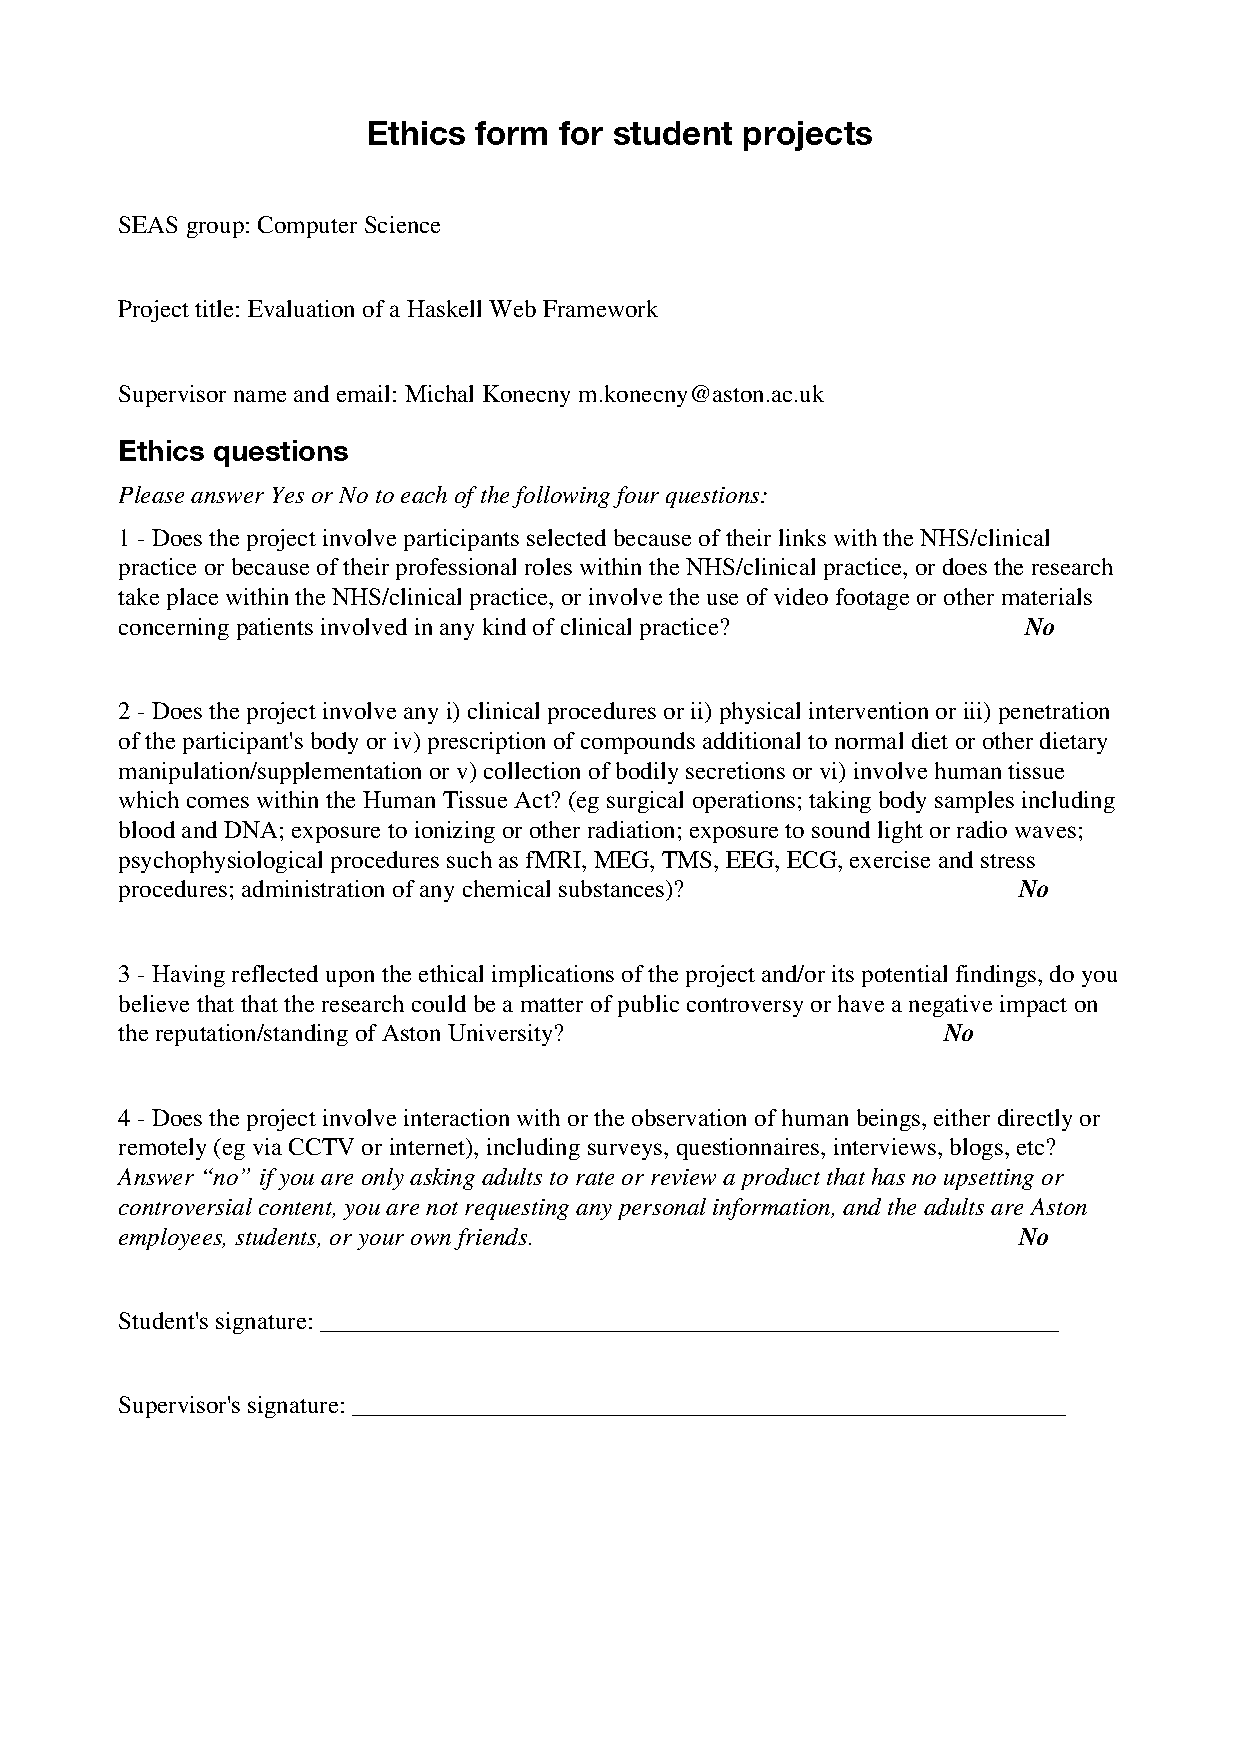
\includepdf[pages=1]{pdf_documents/seas-ethics-student-project-CS-FYP.pdf}

\end{appendices}

\end{document}
